 \documentclass{report}
 
\usepackage[utf8]{inputenc} 
\usepackage[T1]{fontenc}      
\usepackage[top=2.0cm, bottom=3cm, left=3.0cm, right=3.0cm]{geometry}
\usepackage{graphicx}
\usepackage{wrapfig}
\usepackage{amsmath,esint }
\usepackage{amssymb}
\graphicspath{{figures/}{../figures}}

\newcommand*\dif{\mathop{}\!\mathrm{d}}
\newcommand*\diver{\mathop{}\!\mathrm{div}}
\newcommand*\grad{\mathop{}\!\mathrm{grad}}

\begin{document}

\section*{Sillage d'un avion}

On considère le vol d'un avion de chasse se déplaçant dans le sens des $x$ croissants, à une vitesse $v$ sur une droite horizontale $(y=0,z=h)$ alors qu'un observateur est situé au point $O(0,0,0)$. L'avion émet un signal sonore de période $T$. On note $\theta=\vec{Ox},\vec{OA})$ l'inclinaison par rapport à l'horizontale de la direction observateur-avion. Cet angle est supposé varier peu pendant une période $T$.

\begin{itemize}

	\item[$\circ$] L'air a une masse volumique au repos $\rho_0$ et une compressibilité $\chi_s$. Retrouver l'équation d'Alembert caractérisant la propagation des ondes sonores dans l'air, en explicitant la vitesse de propagation $c$ des ondes.

\end{itemize}

On suppose dans un premier temps que l'avion se déplace à une vitesse subsonique, c'est-à-dire $v<c$.

\begin{itemize}

	\item[$\star$] Quelle est la période $T'$ du signal perçu par l'observateur ? Commenter l'expression selon les valeurs prises par $\theta$. Comment s'appelle ce phénomène ?
	
	\item[$\star$] Quelle est la région de l'espace qui peut être atteinte à un instant donné par l'onde sonore provenant de l'avion ?

\end{itemize}

On suppose désormais que l'avion se déplace à une vitesse supersonique, c'est-à-dire $v>c$.

\begin{itemize}

	\item[$\diamond$] Le son émis par l'avion à l'instant $t$ est perçu par l'observateur à l'instant $t'=f(t)$. Déterminer la fonction $f$ si l'avion passe à l'instant $t=0$ à la verticale de l'observateur. Représenter graphiquement $f$.
	
	\item[$\diamond$]  Pourquoi le son perçu est-il particulièrement intense si $\dif t'/\dif t=0$ ? Comment s'appelle ce phénomène ? 
	
	\item[$\diamond$]  On donne $h=1000$m ; $v=500$m.s$^{-1}$ ; $c=340$m.s$^{-1}$. On note $t'_0$ l'instant auquel le bang est perçu par l'observateur et $t_0$ l'instant auquel les sons perçus à l'instant $t'_0$ ont été émis par l'avion. Déterminer $t_0$, $t'_0$ et les positions de l'avion à $t_0$ et $t'_0$. 
	
	\item[$\diamond$] L'observateur entend-il l'avion avant d'entendre le bang ? Quelle est la durée $\Delta t$ d'émission des sons perçus entre $t'_0$ et $t'_0+\Delta t'$ (on pourra effectuer une développement limité de $f(t)$). Calculer $\Delta t$ pour $\Delta t'=0.1$s et commenter.
	
	\item[$\diamond$] Quelle est la région de l'espace qui peut être atteinte à un instant donné par une onde sonore provenant de l'avion ?
	
	\item[$\diamond$] Estimer la vitesse de l'avion en photo ci-dessous.  

\end{itemize}

\begin{figure}[h!]
\centering
		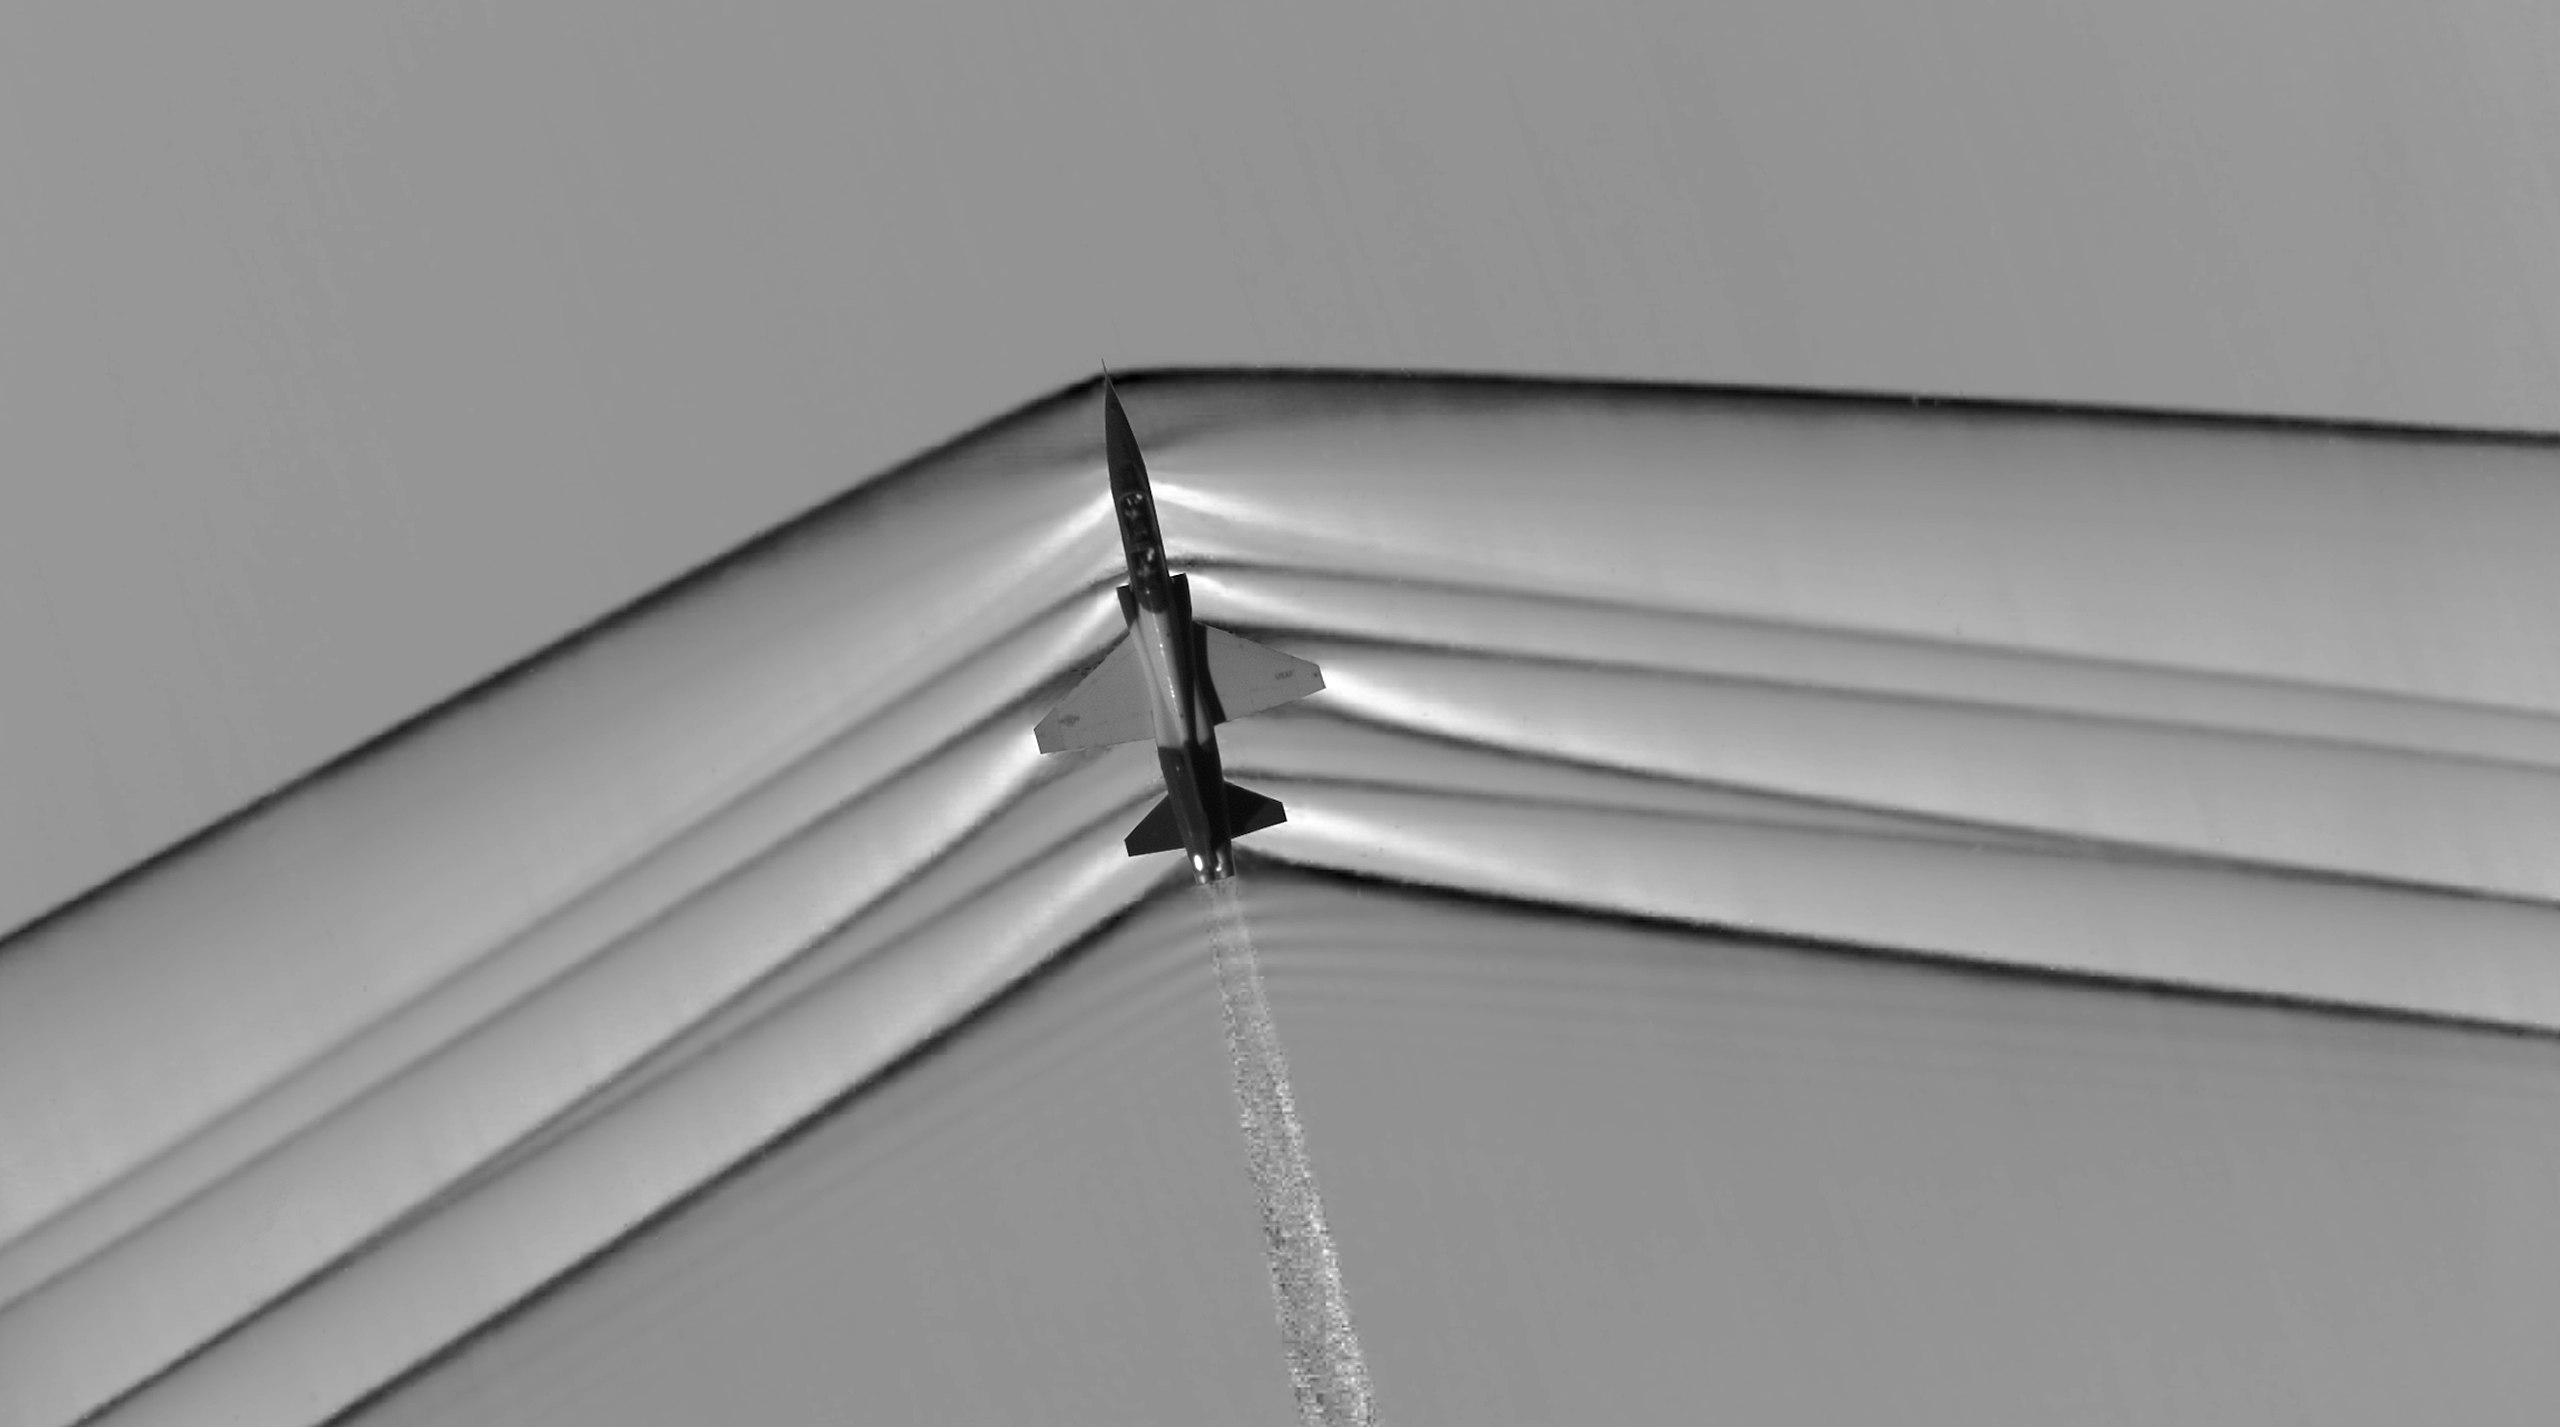
\includegraphics[scale=0.12]{avion.jpg}
\end{figure}

\newpage

\section*{Pavillon acoustique}

Un pavillon acoustique, de symétrie de révolution autour de l'axe $Ox$, contient de l'air de masse volumique $\rho_0$ et de compressibilité $\chi_s$. Une onde s'y propage suivant $Ox$, on suppose que l'approximation acoustique est vérifiée. On note $p(x,t)$ la surpression acoustique et $\Psi(x,t)$ le déplacement longitudinal de la tranche de fluide en $x$ à l'instant $t$. 

\begin{itemize}

\item[$\diamondsuit$] Qu'est-ce que l'approximation acoustique ?

\item[$\diamondsuit$] En reliant la compressibilité $\chi_s=\frac{1}{V}\frac{\partial V}{\partial P}$ à la surpression $p(x,t)$ et au déplacement $\Psi(x,t)$, démontrer la relation suivante :
\begin{align*}
	p(x,t) = -\frac{1}{\chi_s}\left(\frac{\partial \Psi}{\partial x}+\Psi(x,t)\frac{\partial }{\partial x}\left[\ln S(x) \right]  \right)
\end{align*}

\item[$\diamondsuit$] En utilisant l'équation d'Euler (ou bilan de quantité de mouvement sur un fluide), en déduire une relation similaire à une équation d'onde portant sur $\Psi(x,t)$ et sur $p(x,t)$.

\item[$\diamondsuit$] Que devient l'équation de conservation de la masse ? On notera $\mu(x,t)$ la variation de masse volumique par rapport à l'équilibre : $\rho(x,t)=\rho_0+\mu(x,t)$
\end{itemize}

Le pavillon a une allure exponentielle : $S(x)=S_0\exp(ax)$. On suppose que l'onde est une onde plane, progressive et monochromatique : $p(x,t)=p_0\exp\left(j[\omega t-kx] \right)$. On notera la vitesse de déplacement $v(x,t)=\partial\Psi/\partial t$.

\begin{itemize}

\item[$\diamondsuit$]  Quelle est alors l'équation de dispersion ? Montrer qu'il ne peut pas y avoir de propagation en dessous d'une certaine pulsation de coupure $\omega_c$.

\item[$\diamondsuit$] Donner les expression de $v(x,t)$, $p(x,t)$, puis celle de l'énergie acoustique $\varepsilon(x,t)$ et du vecteur de Poyting $\Pi(x,t)$.

\end{itemize}

\newpage

\section*{Impédance acoustique}

On considère une onde acoustique se propageant selon les $x$ croissants dans un milieu 1 et atteignant le milieu 2 en $x=0$. Les milieux 1 et 2 sont caractérisés respectivement par une masse volumique $\rho_1$ et $\rho_2$ et une célérité des ondes acoustiques $c_1$ et $c_2$. 

\subsubsection*{Échographie}

\begin{itemize}
	
	\item[$\spadesuit$] Rappeler l'équation d'Alembert vérifiée par la surpression $p(x,t)$ et la vitesse $v(x,t)$ dans un milieu homogène. Quelles sont les solutions générales ? Qu'appelle t-on les ondes planes progressives monochromatiques ?	
	
	\item[$\spadesuit$] Écrire les relations que vérifient la vitesse et la surpression à l'interface en $x=0$. Que se passe t-il lorsque l'onde arrive de par la gauche sur l'interface $1\longrightarrow2$ pour que ces relations soient vérifiées ? Justifier de l'existence d'une onde réfléchie et transmise.
	
	\item[$\spadesuit$] En déduire les coefficients de réflexion $r$ et de transmission $t$.
	
	\item[$\spadesuit$] Pourquoi dont-on mettre un gel sur entre la sonde et le corps durant une échographie ? 
		
\end{itemize}

\subsubsection*{Isolation phonique}

On suppose qu'il y a désormais une paroi de masse surfacique $\mu$ à l'interface entre les deux milieux, qui sont supposées être identiques ($\rho_1=\rho_2$ et $c_1=c_2$). Cette paroi se meut librement et sans frottement. 

\begin{itemize}
	
	\item[$\clubsuit$] Que deviennent les relations de passage précédentes ? En déduire les coefficients de réflexion et de transmission dans ce cas-là. 
	
	\item[$\clubsuit$] Calculer $T=\mid t\mid^2$ et tracer l'allure de la courbe $G_{db}=20\log\left[T(\omega) \right]$ en fonction de $\log(\omega)$. Quelle est la fréquence de coupure ?
	
	\item[$\clubsuit$] De combien doit être l'épaisseur d'un mur de béton entre deux logements d'un appartement pour que l'atténuation soit atténuée de 50dB à 300Hz ? On donne $\rho_{béton}=2300$kg.m$^{-3}$. 
	
\end{itemize}


\end{document}
